\documentclass[14pt,a4paper,report]{report}
\usepackage[a4paper, mag=1000, left=2.5cm, right=1cm, top=2cm, bottom=2cm, headsep=0.7cm, footskip=1cm]{geometry}
\usepackage[utf8]{inputenc}
\usepackage[english,russian]{babel}
\usepackage{indentfirst}
\usepackage[dvipsnames]{xcolor}
\usepackage[colorlinks]{hyperref}
\usepackage{listings} 
\usepackage{fancyhdr}
\usepackage{caption}
\usepackage{amsmath}
\usepackage{latexsym}
\usepackage{graphicx}
\usepackage{amsmath}
\usepackage{booktabs}
\usepackage{array}
\hypersetup{
	colorlinks = true,
	linkcolor  = black
}

\usepackage{titlesec}
\titleformat{\chapter}
{\Large\bfseries} % format
{}                % label
{0pt}             % sep
{\huge}           % before-code


\DeclareCaptionFont{white}{\color{white}} 

% Listing description
\usepackage{listings} 
\DeclareCaptionFormat{listing}{\colorbox{gray}{\parbox{\textwidth}{#1#2#3}}}
\captionsetup[lstlisting]{format=listing,labelfont=white,textfont=white}
\lstset{ 
	% Listing settings
	inputencoding = utf8,			
	extendedchars = \true, 
	keepspaces = true, 			  	 % Поддержка кириллицы и пробелов в комментариях
	language = Matlab,            	 	 % Язык программирования (для подсветки)
	basicstyle = \small\sffamily, 	 % Размер и начертание шрифта для подсветки кода
	numbers = left,               	 % Где поставить нумерацию строк (слева\справа)
	numberstyle = \tiny,          	 % Размер шрифта для номеров строк
	stepnumber = 1,               	 % Размер шага между двумя номерами строк
	numbersep = 5pt,              	 % Как далеко отстоят номера строк от подсвечиваемого кода
	backgroundcolor = \color{white}, % Цвет фона подсветки - используем \usepackage{color}
	showspaces = false,           	 % Показывать или нет пробелы специальными отступами
	showstringspaces = false,    	 % Показывать или нет пробелы в строках
	showtabs = false,           	 % Показывать или нет табуляцию в строках
	frame = single,              	 % Рисовать рамку вокруг кода
	tabsize = 2,                  	 % Размер табуляции по умолчанию равен 2 пробелам
	captionpos = t,             	 % Позиция заголовка вверху [t] или внизу [b] 
	breaklines = true,           	 % Автоматически переносить строки (да\нет)
	breakatwhitespace = false,   	 % Переносить строки только если есть пробел
	escapeinside = {\%*}{*)}      	 % Если нужно добавить комментарии в коде
}

\begin{document}

\def\contentsname{Содержание}

% Titlepage
\begin{titlepage}
	\begin{center}
		\textsc{Санкт-Петербургский Политехнический 
			Университет Петра Великого\\[5mm]
			Кафедра компьютерных систем и программных технологий}
		
		\vfill
		
		\textbf{Отчёт по лабораторной работе №3\\[3mm]
			Курс: «Методы оптимизации и принятия решений»\\[3mm]
			Тема: «Оптимизация сетей систем массового обслуживания»\\[35mm]
			}
	\end{center}
	
	\hfill
	\begin{minipage}{.5\textwidth}
		Выполнил студент:\\[2mm] 
		Бояркин Никита Сергеевич\\
		Группа: 13541/3\\[5mm]
		
		Проверил:\\[2mm] 
		Сиднев Александр Георгиевич
	\end{minipage}
	\vfill
	\begin{center}
		Санкт-Петербург\\ \the\year\ г.
	\end{center}
\end{titlepage}

% Contents
\tableofcontents
\clearpage

\chapter{Лабораторная работа №3}

\section{Индивидуальное задание}

\subsubsection{Вариант 030}

Задача №2.

\begin{figure}[h!]
	\centering
	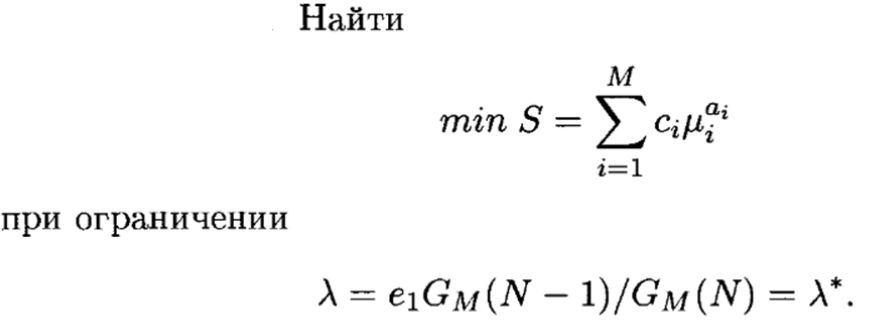
\includegraphics[scale = 0.39]{images/1.png}
	\label{image:1}
\end{figure}

\begin{figure}[h!]
	\centering
	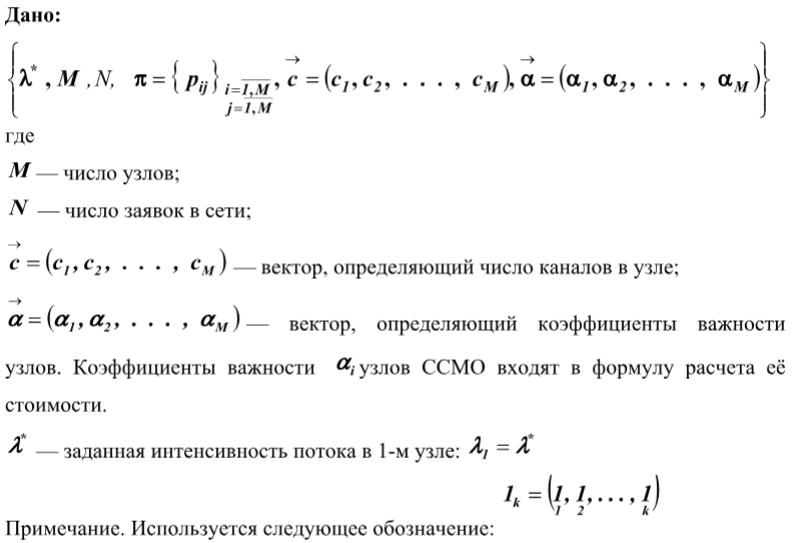
\includegraphics[scale = 0.59]{images/2.png}
	\label{image:2}
\end{figure}

\begin{figure}[h!]
	\centering
	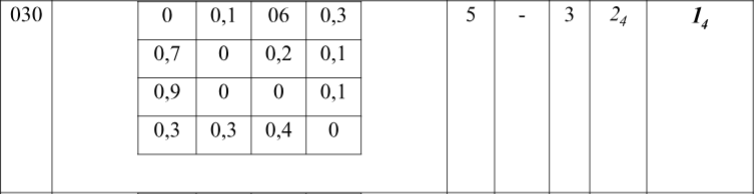
\includegraphics[scale = 0.59]{images/3.png}
	\label{image:3}
\end{figure}

\section{Ход работы}

\subsection{Методика решения простыми итерациями}

Задача оптимизации замкнутой однородной сети сводится к решению системы нелинейных уравнений:

\begin{figure}[h!]
	\centering
	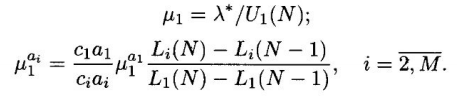
\includegraphics[scale = 0.79]{images/4_r.png}
	\label{image:4r}
\end{figure}

Для многоканальной сети МО используется итерационная процедура расчета среднего числа заявок в очереди. Процедура инициализируется следующими начальными условиями:

\begin{figure}[h!]
	\centering
	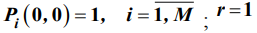
\includegraphics[scale = 0.69]{images/4_0.png}
	\label{image:40}
\end{figure}

Первый шаг процедуры:

\begin{figure}[h!]
	\centering
	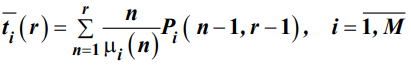
\includegraphics[scale = 0.69]{images/4_1.png}
	\label{image:41}
\end{figure}

\begin{figure}[h!]
	\centering
	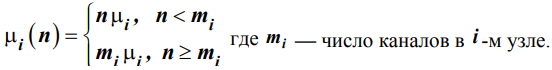
\includegraphics[scale = 0.69]{images/4_m.png}
	\label{image:4m}
\end{figure}

Второй шаг процедуры:

\begin{figure}[h!]
	\centering
	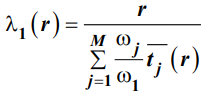
\includegraphics[scale = 0.69]{images/4_2.png}
	\label{image:42}
\end{figure}

Третий шаг процедуры:

\begin{figure}[h!]
	\centering
	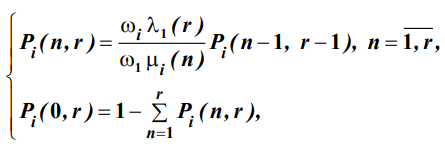
\includegraphics[scale = 0.69]{images/4_3.png}
	\label{image:43}
\end{figure}

После этого значение r увеличивается на единицу до достижения N. В результате работы процедуры формируются значения следующих характеристик:

\begin{figure}[h!]
	\centering
	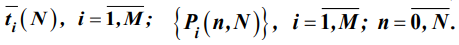
\includegraphics[scale = 0.69]{images/4_4.png}
	\label{image:44}
\end{figure}

\subsection{Решение задачи методом простых итераций}

Разработаем скрипт для расчета результирующего вектора $\mu$ в среде MATLAB:

\lstinputlisting{listings/l1.m}

Итеративная процедура:

\lstinputlisting{listings/fl1.m}

Результат расчета вектора $\mu$:

\lstinputlisting{listings/l1.log}

Алгоритм ожидаемо не сошелся, так как метод простых итераций не рекомендуется к использованию из-за ненадежности в плане сходимости.

\clearpage

\subsection{Методика решения через через нормирующую константу методом Ньютона}

Задача оптимизации замкнутой однородной сети сводится к решению системы нелинейных уравнений:

\begin{figure}[h!]
	\centering
	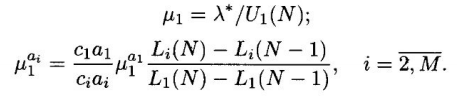
\includegraphics[scale = 0.79]{images/4_r.png}
	\label{image:4rx}
\end{figure}

Тогда интенсивность на выходе i -го узла однородной замкнутой сети СМО:

\begin{figure}[h!]
	\centering
	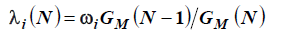
\includegraphics[scale = 0.79]{images/5_1.png}
	\label{image:5_1}
\end{figure}

Среднее число заявок в граничном узле однородной замкнутой сети СМО:

\begin{figure}[h!]
	\centering
	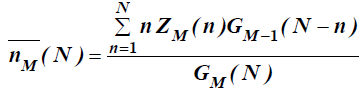
\includegraphics[scale = 0.79]{images/5_2.png}
	\label{image:5_2}
\end{figure}

Методика расчета нормирующей константы:

\begin{figure}[h!]
	\centering
	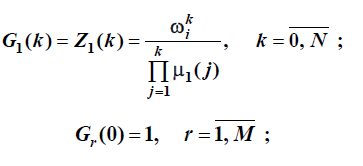
\includegraphics[scale = 0.79]{images/5_4.png}
	\label{image:5_4}
\end{figure}

\begin{figure}[h!]
	\centering
	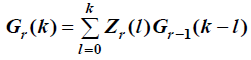
\includegraphics[scale = 0.79]{images/5_5.png}
	\label{image:5_5}
\end{figure}

Алгоритм Ньютона для решения системы нелинейных уравнений (W -- матрица якоби для системы уравнений F):

\begin{figure}[h!]
	\centering
	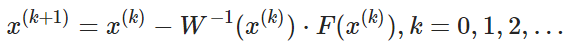
\includegraphics[scale = 0.70]{images/6_1.png}
	\label{image:6_1}
\end{figure}

\subsection{Решение задачи через нормирующую константу методом Ньютона}

Решение задачи через нормирующую константу методом Ньютона c начальным приближением $u=[10, 10, 10, 10]$ и значением ошибки $e=1e^{-6}$:

\lstinputlisting{listings/l3.m}

Расчет нормирующей константы:

\lstinputlisting{listings/gl3.m}

Расчет основных характеристик СМО:

\lstinputlisting{listings/pl3.m}

Результат решения задачи методом Ньютона  c начальным приближением $u=[10, 10, 10, 10]$ и значением ошибки $e=1e^{-6}$:

\lstinputlisting{listings/l3.log}

Алгоритм успешно сходится за 16 итераций. С каждой итерацией алгоритма значения целевых функций стемятся к нулю, результирующая цена также постепенно уменьшается.

\section{Вывод}

Как и ожидалось, алгоритм простых итераций не сходится, поэтому пришлось использовать более надежный алгоритм Ньютона. Модифицированный алгоритм Ньютона чрезвычайно чувствителен к выбору начального приближения, поэтому был использован вариант алгоритма с расчетом матрицы Якоби. Для увеличения производительности данного алгоритма можно подключить пакет MATLAB Parallel Computing Toolbox, который использует MPI для эффективного распараллеливания.

\end{document}